\documentclass[11pt,a4paper,fleqn]{scrartcl}
\usepackage{gram}
\usepackage{amsmath}
\usetikzlibrary{arrows}
\usepackage[p,osf,space]{erewhon}
\usepackage[erewhon,vvarbb,bigdelims]{newtxmath}
\usetikzlibrary{patterns}
\usepackage{svg}
\usepackage{pgfplots}
\pgfplotsset{compat=1.15}
\usepackage{mathrsfs}
\usetikzlibrary{arrows}
\pagecolor{fizikawhite}



\title{FIZIKA-2021 Round-1}
\author{FIZIKA Committee}
\date{August 2021}

\begin{document}
\maketitle
 
\vspace{8mm}
\section{Problem 1}
%% INSP Pr 1
\begin{problem}
There is a system of infinite very long concentric cylindrical shells that have radius $R_1,R_2,R_3,R_4....R_{\infty}$ and having uniformly distributed current given as $I_0,\frac{l_0}{2},\frac{l_0}{4},\frac{l_0}{8},...$ and the outermost shell is having the current of $l_{\infty}$. The current is going inwards in all the shells except the shell at infinity where its going outwards with respect to plane of the paper. Evaluate the ratio $\frac{l_{\infty}}{l_0}$ for which the outermost shell remains stress-free.
\begin{center}
    

\tikzset{every picture/.style={line width=0.75pt}} %set default line width to 0.75pt        
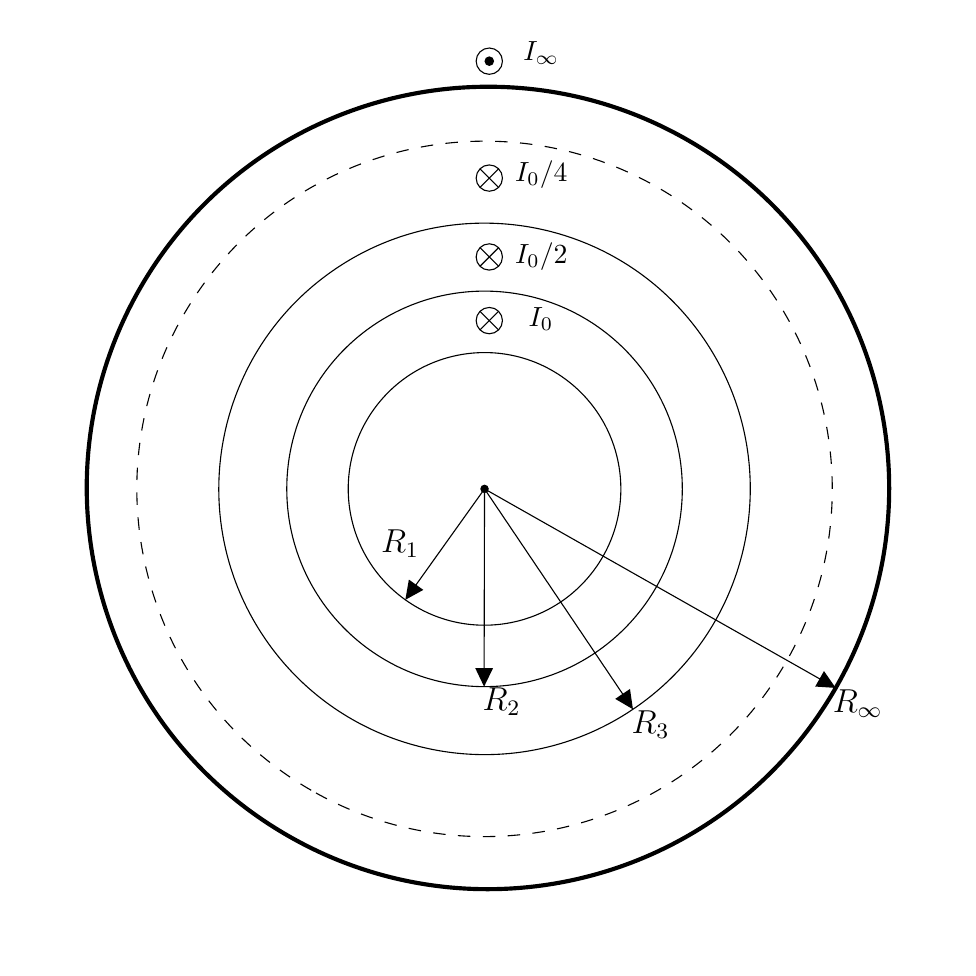
\begin{tikzpicture}[x=0.75pt,y=0.75pt,yscale=-1,xscale=1]
%uncomment if require: \path (0,750); %set diagram left start at 0, and has height of 750

%Shape: Ellipse [id:dp13824326682302956] 
\draw  [line width=1.5]  (242.34,391.51) .. controls (149.81,338.3) and (117.93,220.15) .. (171.14,127.62) .. controls (224.35,35.08) and (342.5,3.2) .. (435.04,56.41) .. controls (527.57,109.62) and (559.45,227.77) .. (506.24,320.31) .. controls (453.03,412.85) and (334.88,444.72) .. (242.34,391.51) -- cycle ;
%Shape: Ellipse [id:dp837502442701394] 
\draw   (230.86,295.92) .. controls (191.36,237.28) and (206.88,157.72) .. (265.53,118.22) .. controls (324.17,78.73) and (403.73,94.25) .. (443.22,152.89) .. controls (482.72,211.54) and (467.2,291.09) .. (408.55,330.59) .. controls (349.91,370.09) and (270.35,354.56) .. (230.86,295.92) -- cycle ;
%Shape: Ellipse [id:dp8448296870986023] 
\draw   (241.76,224.19) .. controls (241.87,171.57) and (284.63,129) .. (337.26,129.12) .. controls (389.88,129.24) and (432.45,172) .. (432.33,224.62) .. controls (432.21,277.25) and (389.45,319.81) .. (336.83,319.69) .. controls (284.2,319.57) and (241.64,276.82) .. (241.76,224.19) -- cycle ;
%Shape: Ellipse [id:dp26024732103447334] 
\draw   (283.6,186.24) .. controls (304.67,156.73) and (345.69,149.89) .. (375.2,170.96) .. controls (404.72,192.04) and (411.56,233.05) .. (390.49,262.57) .. controls (369.41,292.09) and (328.39,298.93) .. (298.88,277.85) .. controls (269.36,256.77) and (262.52,215.76) .. (283.6,186.24) -- cycle ;
%Straight Lines [id:da9435394682627205] 
\draw    (337.04,224.41) -- (503.63,318.83) ;
\draw [shift={(506.24,320.31)}, rotate = 209.54] [fill={rgb, 255:red, 0; green, 0; blue, 0 }  ][line width=0.08]  [draw opacity=0] (8.93,-4.29) -- (0,0) -- (8.93,4.29) -- cycle    ;
%Straight Lines [id:da24753613833187926] 
\draw    (337.04,224.41) -- (406.88,328.1) ;
\draw [shift={(408.55,330.59)}, rotate = 236.04] [fill={rgb, 255:red, 0; green, 0; blue, 0 }  ][line width=0.08]  [draw opacity=0] (8.93,-4.29) -- (0,0) -- (8.93,4.29) -- cycle    ;
%Straight Lines [id:da9326198768496756] 
\draw    (337.04,224.41) -- (336.83,316.69) ;
\draw [shift={(336.83,319.69)}, rotate = 270.13] [fill={rgb, 255:red, 0; green, 0; blue, 0 }  ][line width=0.08]  [draw opacity=0] (8.93,-4.29) -- (0,0) -- (8.93,4.29) -- cycle    ;
%Straight Lines [id:da6485651860835373] 
\draw    (337.04,224.41) -- (300.62,275.41) ;
\draw [shift={(298.88,277.85)}, rotate = 305.53] [fill={rgb, 255:red, 0; green, 0; blue, 0 }  ][line width=0.08]  [draw opacity=0] (8.93,-4.29) -- (0,0) -- (8.93,4.29) -- cycle    ;
%Shape: Ellipse [id:dp17127556547212408] 
\draw  [dash pattern={on 4.5pt off 4.5pt}] (253.54,369.62) .. controls (173.35,323.5) and (145.72,221.11) .. (191.83,140.91) .. controls (237.95,60.71) and (340.34,33.08) .. (420.54,79.2) .. controls (500.74,125.31) and (528.37,227.71) .. (482.25,307.91) .. controls (436.14,388.1) and (333.74,415.73) .. (253.54,369.62) -- cycle ;
%Shape: Ellipse [id:dp12265266084161985] 
\draw   (333,18.33) .. controls (333,14.84) and (335.84,12) .. (339.33,12) .. controls (342.83,12) and (345.67,14.84) .. (345.67,18.33) .. controls (345.67,21.83) and (342.83,24.67) .. (339.33,24.67) .. controls (335.84,24.67) and (333,21.83) .. (333,18.33) -- cycle ;
%Shape: Ellipse [id:dp14680452262194787] 
\draw  [fill={rgb, 255:red, 0; green, 0; blue, 0 }  ,fill opacity=1 ] (337.31,18.33) .. controls (337.31,17.21) and (338.21,16.31) .. (339.33,16.31) .. controls (340.45,16.31) and (341.36,17.21) .. (341.36,18.33) .. controls (341.36,19.45) and (340.45,20.36) .. (339.33,20.36) .. controls (338.21,20.36) and (337.31,19.45) .. (337.31,18.33) -- cycle ;

%Flowchart: Summing Junction [id:dp7499895134813164] 
\draw   (345.67,74.67) .. controls (345.67,71.17) and (342.83,68.33) .. (339.33,68.33) .. controls (335.84,68.33) and (333,71.17) .. (333,74.67) .. controls (333,78.16) and (335.84,81) .. (339.33,81) .. controls (342.83,81) and (345.67,78.16) .. (345.67,74.67) -- cycle ; \draw   (343.81,70.19) -- (334.85,79.15) ; \draw   (334.85,70.19) -- (343.81,79.15) ;
%Flowchart: Summing Junction [id:dp1987512427943714] 
\draw   (345.67,112.67) .. controls (345.67,109.17) and (342.83,106.33) .. (339.33,106.33) .. controls (335.84,106.33) and (333,109.17) .. (333,112.67) .. controls (333,116.16) and (335.84,119) .. (339.33,119) .. controls (342.83,119) and (345.67,116.16) .. (345.67,112.67) -- cycle ; \draw   (343.81,108.19) -- (334.85,117.15) ; \draw   (334.85,108.19) -- (343.81,117.15) ;
%Flowchart: Summing Junction [id:dp06310139127124526] 
\draw   (345.67,143.33) .. controls (345.67,139.84) and (342.83,137) .. (339.33,137) .. controls (335.84,137) and (333,139.84) .. (333,143.33) .. controls (333,146.83) and (335.84,149.67) .. (339.33,149.67) .. controls (342.83,149.67) and (345.67,146.83) .. (345.67,143.33) -- cycle ; \draw   (343.81,138.85) -- (334.85,147.81) ; \draw   (334.85,138.85) -- (343.81,147.81) ;
%Shape: Circle [id:dp8544098462479419] 
\draw  [fill={rgb, 255:red, 0; green, 0; blue, 0 }  ,fill opacity=1 ] (335.29,224.41) .. controls (335.29,225.37) and (336.07,226.16) .. (337.04,226.16) .. controls (338.01,226.16) and (338.79,225.37) .. (338.79,224.41) .. controls (338.79,223.44) and (338.01,222.66) .. (337.04,222.66) .. controls (336.07,222.66) and (335.29,223.44) .. (335.29,224.41) -- cycle ;

% Text Node
\draw (354.54,7.55) node [anchor=north west][inner sep=0.75pt]  [font=\normalsize]  {$I_{\infty}$};
% Text Node
\draw (350.54,104.6) node [anchor=north west][inner sep=0.75pt]  [font=\normalsize]  {$I_{0} /2$};
% Text Node
\draw (350.54,64.91) node [anchor=north west][inner sep=0.75pt]  [font=\normalsize]  {$I_{0} /4$};
% Text Node
\draw (357.04,135.61) node [anchor=north west][inner sep=0.75pt]  [font=\normalsize]  {$I_{0}{}$};
% Text Node
\draw (286.01,243.08) node [anchor=north west][inner sep=0.75pt]  [font=\large]  {$R_{1}$};
% Text Node
\draw (334.89,319.16) node [anchor=north west][inner sep=0.75pt]  [font=\large]  {$R_{2}$};
% Text Node
\draw (406.62,330.05) node [anchor=north west][inner sep=0.75pt]  [font=\large]  {$R_{3}$};
% Text Node
\draw (503.62,319.77) node [anchor=north west][inner sep=0.75pt]  [font=\large]  {$R_{\infty }$};


\end{tikzpicture}

\end{center}


\end{problem}






\begin{solution}
hehehehehehehehehehehehehehehehehehehehehehehehehehehehehehe
\end{solution}



















\section{Problem 2}
%% Anima pr 1
\begin{problem}

Given a peculiar chain of length 1 m, such that it's
linear density varies as $\lambda(x)=x$, where $x$ is distance from
front edge $A$. It is kept on a table with a small hole
such that the edge A starts falling through it and, the height
of table is $h$. ($g=10 m/s$).

%     Figure      %
 \begin{center}
     

\tikzset{every picture/.style={line width=0.75pt}} %set default line width to 0.75pt        

\begin{tikzpicture}[x=0.75pt,y=0.75pt,yscale=-1,xscale=1]

%Shape: Rectangle [id:dp35625532107225033] 
\draw   (106.82,36.24) -- (498.04,36.24) -- (498.04,47.22) -- (106.82,47.22) -- cycle ;
%Shape: Ellipse [id:dp8513224418902086] 
\draw   (294.81,30.5) .. controls (294.81,28.35) and (297.08,26.61) .. (299.88,26.61) .. controls (302.68,26.61) and (304.95,28.35) .. (304.95,30.5) .. controls (304.95,32.64) and (302.68,34.38) .. (299.88,34.38) .. controls (297.08,34.38) and (294.81,32.64) .. (294.81,30.5) -- cycle ;
%Shape: Ellipse [id:dp6183307303752301] 
\draw   (304.95,30.5) .. controls (304.95,28.35) and (307.22,26.61) .. (310.03,26.61) .. controls (312.83,26.61) and (315.1,28.35) .. (315.1,30.5) .. controls (315.1,32.64) and (312.83,34.38) .. (310.03,34.38) .. controls (307.22,34.38) and (304.95,32.64) .. (304.95,30.5) -- cycle ;
%Shape: Ellipse [id:dp054781232838075455] 
\draw   (300.16,23.38) .. controls (300.16,21.23) and (302.43,19.49) .. (305.24,19.49) .. controls (308.04,19.49) and (310.31,21.23) .. (310.31,23.38) .. controls (310.31,25.52) and (308.04,27.26) .. (305.24,27.26) .. controls (302.43,27.26) and (300.16,25.52) .. (300.16,23.38) -- cycle ;
%Shape: Ellipse [id:dp28287015489818557] 
\draw   (310.03,45.19) .. controls (308.16,45.19) and (306.64,42.58) .. (306.64,39.37) .. controls (306.64,36.15) and (308.16,33.54) .. (310.03,33.54) .. controls (311.89,33.54) and (313.41,36.15) .. (313.41,39.37) .. controls (313.41,42.58) and (311.89,45.19) .. (310.03,45.19) -- cycle ;
%Shape: Ellipse [id:dp44157674508282985] 
\draw   (310.03,56.85) .. controls (308.16,56.85) and (306.64,54.24) .. (306.64,51.02) .. controls (306.64,47.8) and (308.16,45.19) .. (310.03,45.19) .. controls (311.89,45.19) and (313.41,47.8) .. (313.41,51.02) .. controls (313.41,54.24) and (311.89,56.85) .. (310.03,56.85) -- cycle ;
%Shape: Ellipse [id:dp7298072780299072] 
\draw   (310.03,68.5) .. controls (308.16,68.5) and (306.64,65.89) .. (306.64,62.67) .. controls (306.64,59.46) and (308.16,56.85) .. (310.03,56.85) .. controls (311.89,56.85) and (313.41,59.46) .. (313.41,62.67) .. controls (313.41,65.89) and (311.89,68.5) .. (310.03,68.5) -- cycle ;
%Shape: Ellipse [id:dp4746873071782114] 
\draw   (310.03,79.51) .. controls (308.16,79.51) and (306.64,76.9) .. (306.64,73.68) .. controls (306.64,70.46) and (308.16,67.85) .. (310.03,67.85) .. controls (311.89,67.85) and (313.41,70.46) .. (313.41,73.68) .. controls (313.41,76.9) and (311.89,79.51) .. (310.03,79.51) -- cycle ;
%Shape: Ellipse [id:dp5004101112922121] 
\draw   (310.03,91.16) .. controls (308.16,91.16) and (306.64,88.55) .. (306.64,85.34) .. controls (306.64,82.12) and (308.16,79.51) .. (310.03,79.51) .. controls (311.89,79.51) and (313.41,82.12) .. (313.41,85.34) .. controls (313.41,88.55) and (311.89,91.16) .. (310.03,91.16) -- cycle ;
%Shape: Ellipse [id:dp11826978989377923] 
\draw   (315.1,30.5) .. controls (315.1,28.35) and (317.37,26.61) .. (320.17,26.61) .. controls (322.97,26.61) and (325.24,28.35) .. (325.24,30.5) .. controls (325.24,32.64) and (322.97,34.38) .. (320.17,34.38) .. controls (317.37,34.38) and (315.1,32.64) .. (315.1,30.5) -- cycle ;
%Shape: Ellipse [id:dp0032854818474798986] 
\draw   (313.55,28.81) .. controls (311.81,28.04) and (311.22,24.98) .. (312.23,21.98) .. controls (313.23,18.98) and (315.46,17.17) .. (317.21,17.94) .. controls (318.95,18.71) and (319.54,21.77) .. (318.53,24.77) .. controls (317.53,27.78) and (315.3,29.59) .. (313.55,28.81) -- cycle ;
%Shape: Ellipse [id:dp3549508174469138] 
\draw   (310.26,21.41) .. controls (308.51,20.67) and (307.86,17.63) .. (308.82,14.6) .. controls (309.78,11.58) and (311.98,9.72) .. (313.73,10.46) .. controls (315.49,11.19) and (316.13,14.24) .. (315.18,17.26) .. controls (314.22,20.28) and (312.02,22.14) .. (310.26,21.41) -- cycle ;
%Shape: Ellipse [id:dp1488068681524506] 
\draw   (289.9,34.65) .. controls (288.14,33.91) and (287.5,30.87) .. (288.45,27.84) .. controls (289.41,24.82) and (291.61,22.96) .. (293.37,23.69) .. controls (295.12,24.43) and (295.77,27.47) .. (294.81,30.5) .. controls (293.85,33.52) and (291.65,35.38) .. (289.9,34.65) -- cycle ;
%Shape: Ellipse [id:dp8120040535459017] 
\draw   (295.53,26.63) .. controls (293.78,25.9) and (293.01,23.25) .. (293.81,20.72) .. controls (294.61,18.19) and (296.68,16.73) .. (298.44,17.46) .. controls (300.19,18.2) and (300.97,20.85) .. (300.16,23.38) .. controls (299.36,25.91) and (297.29,27.37) .. (295.53,26.63) -- cycle ;
%Straight Lines [id:da8996504617539451] 
\draw    (325.67,47.22) -- (325.67,103.84) ;
\draw [shift={(325.67,103.84)}, rotate = 270] [color={rgb, 255:red, 0; green, 0; blue, 0 }  ][line width=0.75]    (0,5.59) -- (0,-5.59)   ;
\draw [shift={(325.67,47.22)}, rotate = 270] [color={rgb, 255:red, 0; green, 0; blue, 0 }  ][line width=0.75]    (0,5.59) -- (0,-5.59)   ;
%Straight Lines [id:da05420889167129239] 
\draw    (131.32,47.22) -- (130.48,151.58) ;
%Straight Lines [id:da17857238934313124] 
\draw    (469.31,47.22) -- (468.46,151.58) ;
%Straight Lines [id:da12137654389665609] 
\draw    (456.63,47.65) -- (455.79,152) ;
%Straight Lines [id:da7658244327929771] 
\draw    (144,47.22) -- (143.15,151.58) ;
%Straight Lines [id:da12150046416595917] 
\draw    (95.83,47.65) -- (94.99,150.73) ;
\draw [shift={(94.99,150.73)}, rotate = 270.47] [color={rgb, 255:red, 0; green, 0; blue, 0 }  ][line width=0.75]    (0,5.59) -- (0,-5.59)   ;
\draw [shift={(95.83,47.65)}, rotate = 270.47] [color={rgb, 255:red, 0; green, 0; blue, 0 }  ][line width=0.75]    (0,5.59) -- (0,-5.59)   ;
%Shape: Ellipse [id:dp057968954440797305] 
\draw   (310.03,102.82) .. controls (308.16,102.82) and (306.64,100.21) .. (306.64,96.99) .. controls (306.64,93.77) and (308.16,91.16) .. (310.03,91.16) .. controls (311.89,91.16) and (313.41,93.77) .. (313.41,96.99) .. controls (313.41,100.21) and (311.89,102.82) .. (310.03,102.82) -- cycle ;
%Shape: Ellipse [id:dp5238375178734451] 
\draw   (283.82,31.1) .. controls (282.07,30.36) and (281.3,27.72) .. (282.1,25.18) .. controls (282.9,22.65) and (284.97,21.2) .. (286.73,21.93) .. controls (288.48,22.66) and (289.26,25.31) .. (288.45,27.84) .. controls (287.65,30.37) and (285.58,31.83) .. (283.82,31.1) -- cycle ;


% Text Node
\draw (329.8,70.04) node [anchor=north west][inner sep=0.75pt]    {$x$};
% Text Node
\draw (75.47,90.32) node [anchor=north west][inner sep=0.75pt]    {$h$};


\end{tikzpicture}

 \end{center}
%    End Figure      %
 
 \vspace{5mm}
A) When $h>1m>x$, then $v(x)=2 \sqrt{x}$.\\
B) When $h>x>1m$, then $x(t)=5t^2+2t+1$.\\
C) When $1 m>h$, $a(t)=$ is dependent of time.\\
D) When $1 m>h$, $a(t)$ is independent of time.
\end{problem}



\section{Problem 3}
%%     JANARDHAN sir pr 1
\begin{problem}
\textbf{A Triangular '$L$' story}; 

The self-inductance of an equilateral triangular loop of side $l$ is $L$ (as shown in figure-$I$). A rhombus of one internal angle $60^{\circ}$ and side '$l$' (as shown in figure-$II$) is placed very close to the triangle so that one of their sides align in the same plane (as shown in figure-$III$) \\

A)If the loop in figure-$I$ were of side '$2l$' instead, then its self-inductance would have been '$2L$'. \\

B) The self-inductance of the loop in figure-$II$ is greater than '$2L$'. \\

C) The mutual inductance between the two loops in figure-$III$ is $\frac{L}{3}$\\

D) The mutual inductance between the two loops in figure-$III$ is $\frac{4L}{3}$\\
\begin{center}
    

\tikzset{every picture/.style={line width=0.75pt}} %set default line width to 0.75pt        

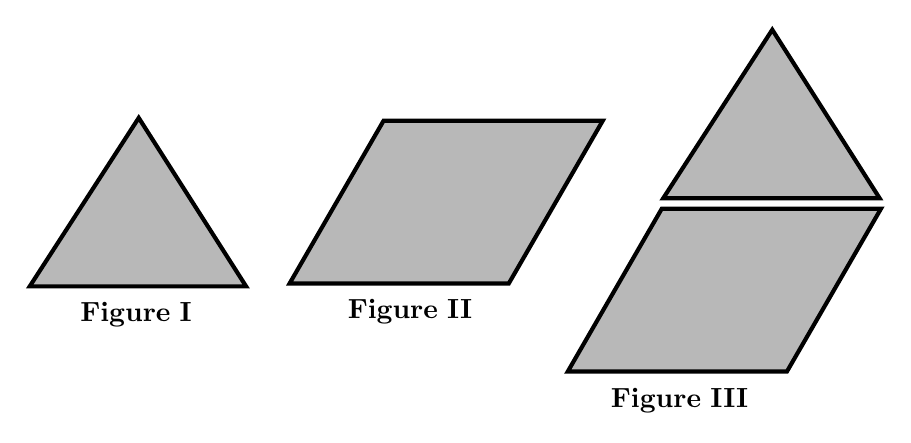
\begin{tikzpicture}[x=0.75pt,y=0.75pt,yscale=-1,xscale=1]
%uncomment if require: \path (0,537); %set diagram left start at 0, and has height of 537

%Shape: Triangle [id:dp4079520034277586] 
\draw  [fill={rgb, 255:red, 0; green, 0; blue, 0 }  ,fill opacity=0.28 ][line width=1.5]  (178.42,51.46) -- (230.14,132.62) -- (125.91,132.62) -- cycle ;
%Shape: Parallelogram [id:dp16119413114025183] 
\draw  [fill={rgb, 255:red, 0; green, 0; blue, 0 }  ,fill opacity=0.28 ][line width=1.5]  (296.37,52.86) -- (401.96,52.86) -- (356.71,131.23) -- (251.11,131.23) -- cycle ;
%Shape: Parallelogram [id:dp9503146048746192] 
\draw  [fill={rgb, 255:red, 0; green, 0; blue, 0 }  ,fill opacity=0.28 ][line width=1.5]  (430.4,95.26) -- (536,95.26) -- (490.74,173.63) -- (385.15,173.63) -- cycle ;
%Shape: Triangle [id:dp3197231943974652] 
\draw  [fill={rgb, 255:red, 0; green, 0; blue, 0 }  ,fill opacity=0.28 ][line width=1.5]  (483.65,9) -- (535.37,90.16) -- (431.13,90.16) -- cycle ;


% Text Node
\draw (149.02,139.08) node [anchor=north west][inner sep=0.75pt]    {$\mathbf{Figure\ I}$};
% Text Node
\draw (277.87,137.62) node [anchor=north west][inner sep=0.75pt]    {$\mathbf{Figure\ II}$};
% Text Node
\draw (404.67,180.6) node [anchor=north west][inner sep=0.75pt]    {$\mathbf{Figure\ III}$};


\end{tikzpicture}

\end{center}



\end{problem}


\section{Problem 4}
\begin{problem}

        
\begin{center}


\tikzset{every picture/.style={line width=0.75pt}} %set default line width to 0.75pt        

\begin{tikzpicture}[x=0.75pt,y=0.75pt,yscale=-1,xscale=1]

\draw   (166,61) -- (283,61) -- (283,178) -- (166,178) -- cycle ;
\draw   (140.5,119.5) .. controls (140.5,73.11) and (178.11,35.5) .. (224.5,35.5) .. controls (270.89,35.5) and (308.5,73.11) .. (308.5,119.5) .. controls (308.5,165.89) and (270.89,203.5) .. (224.5,203.5) .. controls (178.11,203.5) and (140.5,165.89) .. (140.5,119.5) -- cycle ;
\draw   (405,64) -- (522,64) -- (522,181) -- (405,181) -- cycle ;
\draw  [fill={rgb, 255:red, 0; green, 0; blue, 0 }  ,fill opacity=1 ] (222.42,119.5) .. controls (222.42,118.35) and (223.35,117.42) .. (224.5,117.42) .. controls (225.65,117.42) and (226.58,118.35) .. (226.58,119.5) .. controls (226.58,120.65) and (225.65,121.58) .. (224.5,121.58) .. controls (223.35,121.58) and (222.42,120.65) .. (222.42,119.5) -- cycle ;
\draw  [fill={rgb, 255:red, 0; green, 0; blue, 0 }  ,fill opacity=1 ] (461.42,122.5) .. controls (461.42,121.35) and (462.35,120.42) .. (463.5,120.42) .. controls (464.65,120.42) and (465.58,121.35) .. (465.58,122.5) .. controls (465.58,123.65) and (464.65,124.58) .. (463.5,124.58) .. controls (462.35,124.58) and (461.42,123.65) .. (461.42,122.5) -- cycle ;

\draw (395,177.73) node [anchor=north west][inner sep=0.75pt]    {$c$};
\draw (473,101.73) node [anchor=north west][inner sep=0.75pt]    {$o$};
\draw (229.67,99.4) node [anchor=north west][inner sep=0.75pt]    {$o$};


\end{tikzpicture}
    
\end{center}

A uniformly charged non-conducting circular disc has its centre at potential $V$. Now a square plate is cut out of this disc keeping its surface charge density same. The new potential at center and corner are $V_o$ and $V_c$ respectively then\par 
A) \quad $V_o=4V_c$\\
B) \quad $V_o=2V_c$\\
C) \quad $V_o=2V \ln (\sqrt{2}+1)$\\
D) \quad $V_o=\frac{2\sqrt{2}}{\pi}V\ln (\sqrt{2}+1)$\\
\end{problem}



\section{Problem 5}
\begin{problem}

Consider a Bead of mass $m=1Kg$ which is rigidly attached to $2$ mass-less rods at right angles as shown. The lengths of the rods are $2.5m$ and $1m$ as shown. Let's say this arrangement is placed on a rough table with $2$ rigid vertical barriers of $v=5\ m s^{-1}$ perpendicular to the barrier, and it finally comes to rest at the position coordinate $(a,b)$ assuming the initial position to be Origin. Then find the value of
$$4\cdot|b\sqrt{3}-a|$$ 
If 
$$\mu_{table \ and \ bead} = 0.5, g=10m s^{-2}$$
\begin{center}
    

\tikzset{every picture/.style={line width=0.75pt}} %set default line width to 0.75pt        
\boxed{
\begin{tikzpicture}[x=0.75pt,y=0.75pt,yscale=-1,xscale=1]
%uncomment if require: \path (0,356); %set diagram left start at 0, and has height of 356

%Shape: Right Angle [id:dp2423931160285837] 
\draw   (163.31,128.73) -- (163.31,54.35) -- (335.2,54.35) ;
%Shape: Right Angle [id:dp6848218796619385] 
\draw   (163.31,68.4) -- (177.35,68.4) -- (177.35,54.35) ;
%Straight Lines [id:da6965341731217758] 
\draw    (163.31,43.61) -- (335.2,43.61) ;
\draw [shift={(335.2,43.61)}, rotate = 540] [color={rgb, 255:red, 0; green, 0; blue, 0 }  ][line width=0.75]    (0,5.59) -- (0,-5.59)   ;
\draw [shift={(163.31,43.61)}, rotate = 540] [color={rgb, 255:red, 0; green, 0; blue, 0 }  ][line width=0.75]    (0,5.59) -- (0,-5.59)   ;
%Straight Lines [id:da4374043284803446] 
\draw    (150.91,54.35) -- (150.91,128.73) ;
\draw [shift={(150.91,128.73)}, rotate = 270] [color={rgb, 255:red, 0; green, 0; blue, 0 }  ][line width=0.75]    (0,5.59) -- (0,-5.59)   ;
\draw [shift={(150.91,54.35)}, rotate = 270] [color={rgb, 255:red, 0; green, 0; blue, 0 }  ][line width=0.75]    (0,5.59) -- (0,-5.59)   ;
%Straight Lines [id:da40715297571097864] 
\draw    (132.2,188.6) -- (305.2,188.6) ;
%Straight Lines [id:da5701959832709445] 
\draw    (132.2,196.6) -- (288.2,196.6) -- (306.2,196.6) ;
%Straight Lines [id:da06361817267733239] 
\draw    (308.2,186.25) -- (308.2,156.6) ;
\draw [shift={(308.2,153.6)}, rotate = 450] [fill={rgb, 255:red, 0; green, 0; blue, 0 }  ][line width=0.08]  [draw opacity=0] (8.93,-4.29) -- (0,0) -- (8.93,4.29) -- cycle    ;
\draw [shift={(308.2,188.6)}, rotate = 270] [color={rgb, 255:red, 0; green, 0; blue, 0 }  ][line width=0.75]      (0, 0) circle [x radius= 3.35, y radius= 3.35]   ;
%Straight Lines [id:da5724253744031245] 
\draw    (385.53,197.6) -- (385.53,188.6) -- (561.53,187.6) ;
%Straight Lines [id:da9900429843401801] 
\draw    (385.2,197.6) -- (561.53,197.6) ;
%Straight Lines [id:da823718755109442] 
\draw    (297.2,248.47) -- (307.2,192.6) ;
%Straight Lines [id:da2926700586689652] 
\draw    (423,203.4) -- (311.2,188.4) ;

% Text Node
\draw (233.73,25.26) node [anchor=north west][inner sep=0.75pt]    {$2.5m$};
% Text Node
\draw (114.94,84.77) node [anchor=north west][inner sep=0.75pt]    {$1m$};
% Text Node
\draw (306.73,135) node [anchor=north west][inner sep=0.75pt]    {$5m/s$};
% Text Node
\draw (309.4,270.33) node [anchor=north west][inner sep=0.75pt]    {$Top\ View$};


\end{tikzpicture}}

\end{center}
\end{problem}


\section{Problem 6}
\begin{problem}

Consider a very low-resistivity fluid. The magnetic field is at time $t=0$ sec is given by : $\vec{B}$
=$B_0$ $\vec{e_y}$. The velocity field is $\vec{V}= \frac{1}{1+\left(\frac{y}{m}\right)^2} \ \vec{e_x}\  m/s$ always.\\\
What is the magnitude of magnetic field at $(0,1)m$ at $t=1$ second?

$A) B_0 $\\
$B) B_0 /2$\\
$C) \sqrt{3} B_0/2$\\
$D) \sqrt{5} B_0/2$


\end{problem}


\section{Problem 7}
\begin{problem}
Consider the given figure, the blue lines are perfectly reflecting hyperboloid mirrors with coincident foci shown in blue. A beam of light (red) is directed in through an opening at the top left of the system. Two observers $O_1$ and $O_2$ shall receive the light. Find the ratio of the energy density of the multiply reflected beam seen at $O_1$ to that at $O_2$.\\
$a) \quad 0$\\
$b) \quad 1/2$\\
$c) \quad 1$\\
$d) \quad 2$\\
\textbf{Note:} Neglect diffraction and other wave effects.
\begin{center}
    \definecolor{ffwwqq}{rgb}{1,0.4,0}
\definecolor{xdxdff}{rgb}{0.49019607843137253,0.49019607843137253,1}
\definecolor{ffqqqq}{rgb}{1,0,0}
\definecolor{qqqqff}{rgb}{0,0,1}
\begin{tikzpicture}[line cap=round,line join=round,>=triangle 45,x=1cm,y=1cm]
\begin{axis}[
x=1cm,y=1cm,
axis lines=middle,
ymajorgrids=true,
xmajorgrids=true,
xmin=-5.5348681371364865,
xmax=4.361500222676509,
ymin=-3.038270988144141,
ymax=4.96044323257081,
xtick={-4,-2,...,4},
ytick={-2,0,...,4},]
\clip(-5.5348681371364865,-3.038270988144141) rectangle (4.361500222676509,4.96044323257081);
\draw [samples=50,domain=-0.99:0.99,rotate around={0:(0,0)},xshift=0cm,yshift=0cm,line width=2pt,color=qqqqff] plot ({0.75*(1+(\x)^2)/(1-(\x)^2)},{0.565*2*(\x)/(1-(\x)^2)});
\draw [samples=50,domain=-0.99:0.99,rotate around={0:(0,0)},xshift=0cm,yshift=0cm,line width=2pt,color=qqqqff] plot ({0.75*(-1-(\x)^2)/(1-(\x)^2)},{0.565*(-2)*(\x)/(1-(\x)^2)});
\draw [samples=50,domain=-0.99:0.99,rotate around={0:(0,0)},xshift=0cm,yshift=0cm,line width=2pt,color=qqqqff] plot ({0.5*(1+(\x)^2)/(1-(\x)^2)},{0.865*2*(\x)/(1-(\x)^2)});
\draw [samples=50,domain=-0.99:0.99,rotate around={0:(0,0)},xshift=0cm,yshift=0cm,line width=2pt,color=qqqqff] plot ({0.5*(-1-(\x)^2)/(1-(\x)^2)},{0.865*(-2)*(\x)/(1-(\x)^2)});
\draw [->,line width=2.8pt,color=ffqqqq] (-3.857084611176678,4.081996066055657) -- (-3.0669647070714117,2.9531298337946326);
\draw [->,line width=2.8pt,color=ffqqqq] (-2.609314348408259,4.772247777142751) -- (-2.1224665620339076,3.3285532816392123);
\draw [line width=3.2pt,dash pattern=on 1pt off 1pt,color=ffwwqq] (-3.0669647070714117,2.9531298337946326)-- (-1,0);
\draw [line width=3.2pt,dash pattern=on 1pt off 1pt,color=ffwwqq] (-1,0)-- (-2.1224665620339076,3.3285532816392123);
\draw [->,line width=2.8pt,color=ffqqqq] (-3.4550340500135075,4.414219286214349) -- (-2.720067816314126,3.0927296215417623);
\draw [->,line width=2.8pt,color=ffqqqq] (-2.972519219091779,4.551647769246634) -- (-2.4218894093222323,3.281052825957698);
\begin{scriptsize}
\draw [fill=black] (-0.75,-0.5) circle (2pt);
\draw[color=black] (-0.14797896808363964,-0.26830809155726726) node {\textbf{$O_1(-0.75,-0.5)$}};
\draw [fill=black] (-0.75,0.5) circle (2pt);
\draw[color=black] (-0.1887887345158581,0.7315311860321017) node {\textbf{$O_2(-0.75,0.5)$}};
\draw [fill=xdxdff] (-1,0) circle (2.5pt);
\end{scriptsize}
\end{axis}
\end{tikzpicture}
\end{center}

\end{problem}



\section{Problem 8}
\begin{problem}
A disc of mass $M$, and radius $R$ is free to rotate about a fixed axis perpendicular to its surface and passing through its Centre of Mass. It is bound by a light spring, with a natural length of $L$. At its natural length, one end of the spring is connected to a fixed wall located at a distance of $L$ from the disc, and the other end is connected to the disc. The disc is rotated so that the spring forms a tangent to it and is released from that position. Samar sticks a ring of mass $16M$ and radius $R/N$ on the disc with the same fixed axis. He sticks this ring when the disc has maximum angular velocity and ensures he doesn't change its angular velocity. The spring snaps at a length $3\sqrt{L^2 + 2LR} - 2L$. You can assume that the spring exerts a force tangential to it at any given point. Friction is negligible everywhere. If $N\geq1$, find the minimum $N$ so the spring does not snap.
\vspace{6mm}
\begin{center}
    

\tikzset{every picture/.style={line width=0.75pt}} %set default line width to 0.75pt        

\begin{tikzpicture}[x=0.75pt,y=0.75pt,yscale=-1,xscale=1]
%uncomment if require: \path (0,537); %set diagram left start at 0, and has height of 537

%Straight Lines [id:da08727876157803438] 
\draw [line width=1.5]    (111,30) -- (518,30) ;
%Shape: Spring [id:dp23811323445365273] 
\draw   (328.32,40.9) .. controls (338.09,58.35) and (302.22,76.15) .. (296.84,66.55) .. controls (291.47,56.95) and (327.34,39.15) .. (337.12,56.6) .. controls (346.89,74.05) and (311.01,91.85) .. (305.64,82.26) .. controls (300.26,72.66) and (336.14,54.86) .. (345.91,72.31) .. controls (355.68,89.76) and (319.81,107.56) .. (314.43,97.96) .. controls (309.06,88.36) and (344.93,70.56) .. (354.71,88.01) .. controls (364.48,105.46) and (328.6,123.26) .. (323.23,113.67) .. controls (317.85,104.07) and (353.73,86.27) .. (363.5,103.72) .. controls (373.27,121.17) and (337.4,138.97) .. (332.02,129.37) .. controls (326.65,119.77) and (362.52,101.97) .. (372.3,119.42) .. controls (382.07,136.87) and (346.19,154.67) .. (340.82,145.08) .. controls (335.44,135.48) and (371.32,117.68) .. (381.09,135.13) .. controls (382.23,137.15) and (382.75,139.18) .. (382.77,141.17) ;
%Straight Lines [id:da6664577629638426] 
\draw    (324.6,31) -- (329,42.8) ;
%Straight Lines [id:da9213650211555284] 
\draw    (382.2,137.4) -- (394.6,217) ;
%Shape: Circle [id:dp9435150427604724] 
\draw   (204.2,258.1) .. controls (204.2,203.26) and (248.66,158.8) .. (303.5,158.8) .. controls (358.34,158.8) and (402.8,203.26) .. (402.8,258.1) .. controls (402.8,312.94) and (358.34,357.4) .. (303.5,357.4) .. controls (248.66,357.4) and (204.2,312.94) .. (204.2,258.1) -- cycle ;




\end{tikzpicture}

\end{center}
\end{problem}


\section{Problem 9}
\begin{problem}
A potential difference of $\displaystyle V{o}$ initiates the flow of steady current from top to bottom of the conductor (conductivity of medium is $\displaystyle \sigma $). Atharva broke the conductor and a hemispherical bump is generated in the conductor. Now he initiates the flow of current, he found that current flowing into that hemispherical bump of radius R is $\displaystyle k\pi \sigma R^{2}\frac{V{o}}{d}$ , Assuming $\displaystyle d\gg R$ find the value of $k$? 
\vspace{10mm}
\begin{center}
    

\tikzset{every picture/.style={line width=0.75pt}} %set default line width to 0.75pt        

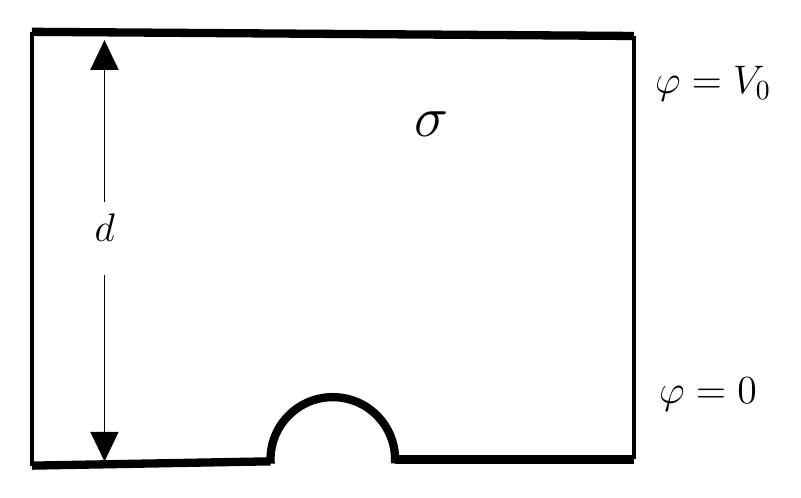
\begin{tikzpicture}[x=0.75pt,y=0.75pt,yscale=-1,xscale=1]
%uncomment if require: \path (0,537); %set diagram left start at 0, and has height of 537

%Straight Lines [id:da013965873027830922] 
\draw [line width=1.5]    (146,23) -- (146,232) ;
%Straight Lines [id:da26039574445576497] 
\draw [line width=1.5]    (436,25) -- (436,229) ;
%Straight Lines [id:da8920404489161631] 
\draw [line width=3]    (436,25) -- (146,23) ;
%Shape: Arc [id:dp740455878657255] 
\draw  [draw opacity=0][line width=3]  (261.07,231.07) .. controls (261.02,230.38) and (261,229.69) .. (261,229) .. controls (261,212.43) and (274.43,199) .. (291,199) .. controls (307.57,199) and (321,212.43) .. (321,229) .. controls (321,229.65) and (320.98,230.29) .. (320.94,230.93) -- (291,229) -- cycle ; \draw  [line width=3]  (261.07,231.07) .. controls (261.02,230.38) and (261,229.69) .. (261,229) .. controls (261,212.43) and (274.43,199) .. (291,199) .. controls (307.57,199) and (321,212.43) .. (321,229) .. controls (321,229.65) and (320.98,230.29) .. (320.94,230.93) ;
%Straight Lines [id:da3028129433938429] 
\draw [line width=3]    (261.01,229.94) -- (146,232) ;
%Straight Lines [id:da5385350556293031] 
\draw [line width=3]    (436,229) -- (321,229) ;

%Straight Lines [id:da11953546043815222] 
\draw    (181,105) -- (181,30) ;
\draw [shift={(181,27)}, rotate = 450] [fill={rgb, 255:red, 0; green, 0; blue, 0 }  ][line width=0.08]  [draw opacity=0] (14.29,-6.86) -- (0,0) -- (14.29,6.86) -- cycle    ;
%Straight Lines [id:da04514608560286959] 
\draw    (181,140) -- (181,227) ;
\draw [shift={(181,230)}, rotate = 270] [fill={rgb, 255:red, 0; green, 0; blue, 0 }  ][line width=0.08]  [draw opacity=0] (14.29,-6.86) -- (0,0) -- (14.29,6.86) -- cycle    ;

% Text Node
\draw (175,109.4) node [anchor=north west][inner sep=0.75pt]  [font=\Large]  {$d$};
% Text Node
\draw (329,60.4) node [anchor=north west][inner sep=0.75pt]  [font=\huge]  {$\sigma $};
% Text Node
\draw (445,38.4) node [anchor=north west][inner sep=0.75pt]  [font=\Large]  {$\varphi =V_{0}$};
% Text Node
\draw (447,188.4) node [anchor=north west][inner sep=0.75pt]  [font=\Large]  {$\varphi =0$};


\end{tikzpicture}

\end{center}
\end{problem}



\section{Problem 10}
\begin{problem}

Samar and Aayush live in a strange magical world. For doing magic, they need a perfect cylindrical wand. Samar and Aayush are sworn enemies and in a previous fight between them, Samar's wand broke so he made a new wand. He intended to make a perfect wand, but while using the charm ``Rictumsempra", Aayush disturbed him and as a result, the radius of Samar's wand became:

$R(x)=R_0+r\sin^2 \frac{2 \pi x}{a}$ \ and length of the wand is $\ell$.

Somehow this wand reached Aditya in the Muggle world and Aditya wanted to calculate the resistance of the wand. He found the resistivity of the wand's material to be $\rho_0$. Can you determine the resistance of the wand that Aditya found. 
Assume that $r\ll R$ and $a\ll l$
\vspace{5mm}

\textbf{a)}The resistance of wand determined by Aditya will be $\frac{\rho l}{\pi R_o^2}$ \newline 
\textbf{b)}The resistance of wand determined by Aditya will be $\frac{\rho l}{\pi R_o^2}\qty(1+\frac{r^2}{R_o^2})$ 
\newline \textbf{c)}The resistance of wand determined by Aditya will be $\frac{\rho l}{\pi R_o^2}\qty(1-\frac{r^2}{R_o^2})$ 
\newline \textbf{d)}The resistance of wand determined by Aditya will be $\frac{\rho l}{\pi R_o^2}\qty(1-\frac{r}{R_o})$
\vspace{10mm}
\begin{center}
    

\tikzset{every picture/.style={line width=0.75pt}} %set default line width to 0.75pt        

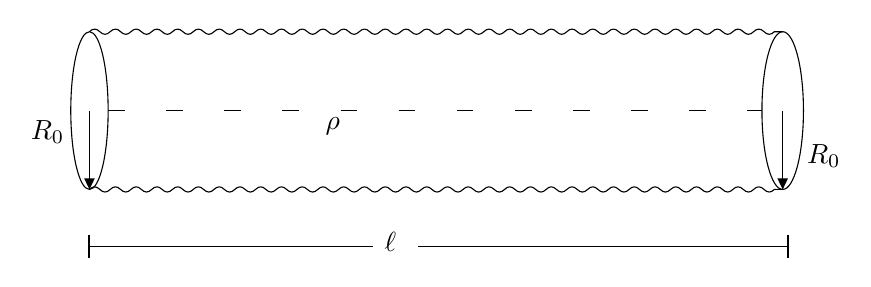
\begin{tikzpicture}[x=0.75pt,y=0.75pt,yscale=-1,xscale=1]
%uncomment if require: \path (0,448); %set diagram left start at 0, and has height of 448

%Shape: Ellipse [id:dp3730606810567325] 
\draw   (95.5,170) .. controls (95.5,149.01) and (99.53,132) .. (104.5,132) .. controls (109.47,132) and (113.5,149.01) .. (113.5,170) .. controls (113.5,190.99) and (109.47,208) .. (104.5,208) .. controls (99.53,208) and (95.5,190.99) .. (95.5,170) -- cycle ;
%Shape: Ellipse [id:dp6366590494916369] 
\draw   (428.5,170) .. controls (428.5,149.01) and (432.98,132) .. (438.5,132) .. controls (444.02,132) and (448.5,149.01) .. (448.5,170) .. controls (448.5,190.99) and (444.02,208) .. (438.5,208) .. controls (432.98,208) and (428.5,190.99) .. (428.5,170) -- cycle ;
%Straight Lines [id:da17407338648740622] 
\draw    (104.5,132) .. controls (106.17,130.33) and (107.83,130.33) .. (109.5,132) .. controls (111.17,133.67) and (112.83,133.67) .. (114.5,132) .. controls (116.17,130.33) and (117.83,130.33) .. (119.5,132) .. controls (121.17,133.67) and (122.83,133.67) .. (124.5,132) .. controls (126.17,130.33) and (127.83,130.33) .. (129.5,132) .. controls (131.17,133.67) and (132.83,133.67) .. (134.5,132) .. controls (136.17,130.33) and (137.83,130.33) .. (139.5,132) .. controls (141.17,133.67) and (142.83,133.67) .. (144.5,132) .. controls (146.17,130.33) and (147.83,130.33) .. (149.5,132) .. controls (151.17,133.67) and (152.83,133.67) .. (154.5,132) .. controls (156.17,130.33) and (157.83,130.33) .. (159.5,132) .. controls (161.17,133.67) and (162.83,133.67) .. (164.5,132) .. controls (166.17,130.33) and (167.83,130.33) .. (169.5,132) .. controls (171.17,133.67) and (172.83,133.67) .. (174.5,132) .. controls (176.17,130.33) and (177.83,130.33) .. (179.5,132) .. controls (181.17,133.67) and (182.83,133.67) .. (184.5,132) .. controls (186.17,130.33) and (187.83,130.33) .. (189.5,132) .. controls (191.17,133.67) and (192.83,133.67) .. (194.5,132) .. controls (196.17,130.33) and (197.83,130.33) .. (199.5,132) .. controls (201.17,133.67) and (202.83,133.67) .. (204.5,132) .. controls (206.17,130.33) and (207.83,130.33) .. (209.5,132) .. controls (211.17,133.67) and (212.83,133.67) .. (214.5,132) .. controls (216.17,130.33) and (217.83,130.33) .. (219.5,132) .. controls (221.17,133.67) and (222.83,133.67) .. (224.5,132) .. controls (226.17,130.33) and (227.83,130.33) .. (229.5,132) .. controls (231.17,133.67) and (232.83,133.67) .. (234.5,132) .. controls (236.17,130.33) and (237.83,130.33) .. (239.5,132) .. controls (241.17,133.67) and (242.83,133.67) .. (244.5,132) .. controls (246.17,130.33) and (247.83,130.33) .. (249.5,132) .. controls (251.17,133.67) and (252.83,133.67) .. (254.5,132) .. controls (256.17,130.33) and (257.83,130.33) .. (259.5,132) .. controls (261.17,133.67) and (262.83,133.67) .. (264.5,132) .. controls (266.17,130.33) and (267.83,130.33) .. (269.5,132) .. controls (271.17,133.67) and (272.83,133.67) .. (274.5,132) .. controls (276.17,130.33) and (277.83,130.33) .. (279.5,132) .. controls (281.17,133.67) and (282.83,133.67) .. (284.5,132) .. controls (286.17,130.33) and (287.83,130.33) .. (289.5,132) .. controls (291.17,133.67) and (292.83,133.67) .. (294.5,132) .. controls (296.17,130.33) and (297.83,130.33) .. (299.5,132) .. controls (301.17,133.67) and (302.83,133.67) .. (304.5,132) .. controls (306.17,130.33) and (307.83,130.33) .. (309.5,132) .. controls (311.17,133.67) and (312.83,133.67) .. (314.5,132) .. controls (316.17,130.33) and (317.83,130.33) .. (319.5,132) .. controls (321.17,133.67) and (322.83,133.67) .. (324.5,132) .. controls (326.17,130.33) and (327.83,130.33) .. (329.5,132) .. controls (331.17,133.67) and (332.83,133.67) .. (334.5,132) .. controls (336.17,130.33) and (337.83,130.33) .. (339.5,132) .. controls (341.17,133.67) and (342.83,133.67) .. (344.5,132) .. controls (346.17,130.33) and (347.83,130.33) .. (349.5,132) .. controls (351.17,133.67) and (352.83,133.67) .. (354.5,132) .. controls (356.17,130.33) and (357.83,130.33) .. (359.5,132) .. controls (361.17,133.67) and (362.83,133.67) .. (364.5,132) .. controls (366.17,130.33) and (367.83,130.33) .. (369.5,132) .. controls (371.17,133.67) and (372.83,133.67) .. (374.5,132) .. controls (376.17,130.33) and (377.83,130.33) .. (379.5,132) .. controls (381.17,133.67) and (382.83,133.67) .. (384.5,132) .. controls (386.17,130.33) and (387.83,130.33) .. (389.5,132) .. controls (391.17,133.67) and (392.83,133.67) .. (394.5,132) .. controls (396.17,130.33) and (397.83,130.33) .. (399.5,132) .. controls (401.17,133.67) and (402.83,133.67) .. (404.5,132) .. controls (406.17,130.33) and (407.83,130.33) .. (409.5,132) .. controls (411.17,133.67) and (412.83,133.67) .. (414.5,132) .. controls (416.17,130.33) and (417.83,130.33) .. (419.5,132) .. controls (421.17,133.67) and (422.83,133.67) .. (424.5,132) .. controls (426.17,130.33) and (427.83,130.33) .. (429.5,132) .. controls (431.17,133.67) and (432.83,133.67) .. (434.5,132) -- (438.5,132) -- (438.5,132) ;
%Straight Lines [id:da41974809031947014] 
\draw    (104.5,208) .. controls (106.17,206.33) and (107.83,206.33) .. (109.5,208) .. controls (111.17,209.67) and (112.83,209.67) .. (114.5,208) .. controls (116.17,206.33) and (117.83,206.33) .. (119.5,208) .. controls (121.17,209.67) and (122.83,209.67) .. (124.5,208) .. controls (126.17,206.33) and (127.83,206.33) .. (129.5,208) .. controls (131.17,209.67) and (132.83,209.67) .. (134.5,208) .. controls (136.17,206.33) and (137.83,206.33) .. (139.5,208) .. controls (141.17,209.67) and (142.83,209.67) .. (144.5,208) .. controls (146.17,206.33) and (147.83,206.33) .. (149.5,208) .. controls (151.17,209.67) and (152.83,209.67) .. (154.5,208) .. controls (156.17,206.33) and (157.83,206.33) .. (159.5,208) .. controls (161.17,209.67) and (162.83,209.67) .. (164.5,208) .. controls (166.17,206.33) and (167.83,206.33) .. (169.5,208) .. controls (171.17,209.67) and (172.83,209.67) .. (174.5,208) .. controls (176.17,206.33) and (177.83,206.33) .. (179.5,208) .. controls (181.17,209.67) and (182.83,209.67) .. (184.5,208) .. controls (186.17,206.33) and (187.83,206.33) .. (189.5,208) .. controls (191.17,209.67) and (192.83,209.67) .. (194.5,208) .. controls (196.17,206.33) and (197.83,206.33) .. (199.5,208) .. controls (201.17,209.67) and (202.83,209.67) .. (204.5,208) .. controls (206.17,206.33) and (207.83,206.33) .. (209.5,208) .. controls (211.17,209.67) and (212.83,209.67) .. (214.5,208) .. controls (216.17,206.33) and (217.83,206.33) .. (219.5,208) .. controls (221.17,209.67) and (222.83,209.67) .. (224.5,208) .. controls (226.17,206.33) and (227.83,206.33) .. (229.5,208) .. controls (231.17,209.67) and (232.83,209.67) .. (234.5,208) .. controls (236.17,206.33) and (237.83,206.33) .. (239.5,208) .. controls (241.17,209.67) and (242.83,209.67) .. (244.5,208) .. controls (246.17,206.33) and (247.83,206.33) .. (249.5,208) .. controls (251.17,209.67) and (252.83,209.67) .. (254.5,208) .. controls (256.17,206.33) and (257.83,206.33) .. (259.5,208) .. controls (261.17,209.67) and (262.83,209.67) .. (264.5,208) .. controls (266.17,206.33) and (267.83,206.33) .. (269.5,208) .. controls (271.17,209.67) and (272.83,209.67) .. (274.5,208) .. controls (276.17,206.33) and (277.83,206.33) .. (279.5,208) .. controls (281.17,209.67) and (282.83,209.67) .. (284.5,208) .. controls (286.17,206.33) and (287.83,206.33) .. (289.5,208) .. controls (291.17,209.67) and (292.83,209.67) .. (294.5,208) .. controls (296.17,206.33) and (297.83,206.33) .. (299.5,208) .. controls (301.17,209.67) and (302.83,209.67) .. (304.5,208) .. controls (306.17,206.33) and (307.83,206.33) .. (309.5,208) .. controls (311.17,209.67) and (312.83,209.67) .. (314.5,208) .. controls (316.17,206.33) and (317.83,206.33) .. (319.5,208) .. controls (321.17,209.67) and (322.83,209.67) .. (324.5,208) .. controls (326.17,206.33) and (327.83,206.33) .. (329.5,208) .. controls (331.17,209.67) and (332.83,209.67) .. (334.5,208) .. controls (336.17,206.33) and (337.83,206.33) .. (339.5,208) .. controls (341.17,209.67) and (342.83,209.67) .. (344.5,208) .. controls (346.17,206.33) and (347.83,206.33) .. (349.5,208) .. controls (351.17,209.67) and (352.83,209.67) .. (354.5,208) .. controls (356.17,206.33) and (357.83,206.33) .. (359.5,208) .. controls (361.17,209.67) and (362.83,209.67) .. (364.5,208) .. controls (366.17,206.33) and (367.83,206.33) .. (369.5,208) .. controls (371.17,209.67) and (372.83,209.67) .. (374.5,208) .. controls (376.17,206.33) and (377.83,206.33) .. (379.5,208) .. controls (381.17,209.67) and (382.83,209.67) .. (384.5,208) .. controls (386.17,206.33) and (387.83,206.33) .. (389.5,208) .. controls (391.17,209.67) and (392.83,209.67) .. (394.5,208) .. controls (396.17,206.33) and (397.83,206.33) .. (399.5,208) .. controls (401.17,209.67) and (402.83,209.67) .. (404.5,208) .. controls (406.17,206.33) and (407.83,206.33) .. (409.5,208) .. controls (411.17,209.67) and (412.83,209.67) .. (414.5,208) .. controls (416.17,206.33) and (417.83,206.33) .. (419.5,208) .. controls (421.17,209.67) and (422.83,209.67) .. (424.5,208) .. controls (426.17,206.33) and (427.83,206.33) .. (429.5,208) .. controls (431.17,209.67) and (432.83,209.67) .. (434.5,208) -- (438.5,208) -- (438.5,208) ;
%Straight Lines [id:da25370343879441815] 
\draw    (104.5,170) -- (104.5,205) ;
\draw [shift={(104.5,208)}, rotate = 270] [fill={rgb, 255:red, 0; green, 0; blue, 0 }  ][line width=0.08]  [draw opacity=0] (5.36,-2.57) -- (0,0) -- (5.36,2.57) -- cycle    ;
%Straight Lines [id:da5271078752233052] 
\draw    (438.5,170) -- (438.5,205) ;
\draw [shift={(438.5,208)}, rotate = 270] [fill={rgb, 255:red, 0; green, 0; blue, 0 }  ][line width=0.08]  [draw opacity=0] (5.36,-2.57) -- (0,0) -- (5.36,2.57) -- cycle    ;
%Straight Lines [id:da7195748473414709] 
\draw  [dash pattern={on 6pt off 15pt}]  (113.5,170) -- (428.5,170) ;
%Straight Lines [id:da11786269928499071] 
\draw    (263,235.5) -- (441,235.5) ;
\draw [shift={(441,235.5)}, rotate = 180] [color={rgb, 255:red, 0; green, 0; blue, 0 }  ][line width=0.75]    (0,5.59) -- (0,-5.59)   ;
%Straight Lines [id:da9998401002718653] 
\draw    (241,235.5) -- (104.5,235.5) ;
\draw [shift={(104.5,235.5)}, rotate = 360] [color={rgb, 255:red, 0; green, 0; blue, 0 }  ][line width=0.75]    (0,5.59) -- (0,-5.59)   ;

% Text Node
\draw (75,173.4) node [anchor=north west][inner sep=0.75pt]    {$R_{0}$};
% Text Node
\draw (449,184.9) node [anchor=north west][inner sep=0.75pt]    {$R_{0}$};
% Text Node
\draw (217,171.9) node [anchor=north west][inner sep=0.75pt]    {$\rho $};
% Text Node
\draw (245.5,227.4) node [anchor=north west][inner sep=0.75pt]    {$\ell $};


\end{tikzpicture}

\end{center}

\end{problem}

 

\end{document}